\documentclass[runningheads]{llncs}

\usepackage[T1]{fontenc}
\usepackage[utf8]{inputenc}
\usepackage{graphicx}
\usepackage{amsmath,amssymb,amsfonts}
\usepackage{booktabs}
\usepackage{array}
\usepackage{float}
\usepackage{xcolor}
\usepackage{hyperref}

\hypersetup{
    colorlinks=true,
    linkcolor=blue!60!black,
    citecolor=blue!60!black,
    urlcolor=blue!60!black
}
\renewcommand\UrlFont{\color{blue}\rmfamily}
\urlstyle{rm}

\begin{document}

\title{Investiga\c{c}\~{a}o Emp\'{i}rica, Conex\~{o}es Residuais e Mecanismos de Aten\c{c}\~{a}o em Redes Neurais Convolucionais para Classifica\c{c}\~{a}o no CIFAR-10}
\titlerunning{Investiga\c{c}\~{a}o Emp\'{i}rica e Otimiza\c{c}\~{a}o Arquitetural de CNNs no CIFAR-10}

\author{Jos\'{e} Alb\'{e}rico Rocha da Silva\inst{1}}
\authorrunning{J. A. R. da Silva}

\institute{Universidade Federal Rural de Pernambuco (UFRPE)\\
Departamento de Computa\c{c}\~{a}o -- T\'{o}picos Avan\c{c}ados em Intelig\^{e}ncia Artificial (2026.2)\\
Recife - PE, Brasil\\
\email{jose.alberico@ufrpe.br}\\
\url{https://github.com/albericolx/Topicos_Avancados_IA}}

\maketitle

\begin{abstract}
Este artigo cient\'{i}fico formaliza a investiga\c{c}\~{a}o emp\'{i}rica, reprodu\c{c}\~{a}o de refer\^{e}ncia e extens\~{a}o arquitetural de uma rede neural convolucional moderna (\textit{Convolutional Neural Network} -- CNN) aplicada \`{a} classifica\c{c}\~{a}o de imagens naturais no \textit{benchmark} can\^{o}nico CIFAR-10, correspondente ao Artefato \texttt{[5] arquitetura tech report} (\texttt{arq$\cdot$p}) da disciplina T\'{o}picos Avan\c{c}ados em Intelig\^{e}ncia Artificial (UFRPE 2026.2). Inicialmente, reproduz-se fielmente o modelo basal de Dizabadi (\textit{arXiv:2604.23861, 2026}), composto por 6 camadas convolucionais $3 \times 3$, 7 camadas de normaliza\c{c}\~{a}o em lote (\textit{Batch Normalization}), subamostragem por \textit{Max Pooling} e regulariza\c{c}\~{a}o estoc\'{a}stica por \textit{Dropout}, totalizando exatamente $552.874$ par\^{a}metros. A partir do diagn\'{o}stico de duas lacunas fundamentais na literatura original -- o colapso severo no aprendizado ao aumentar a profundidade para 8 convolu\c{c}\~{o}es ($83{,}42\% \to 70{,}66\%$) decorrente do desvanecimento de gradientes e o sobreajuste estrutural oriundo do treinamento com dados puramente est\'{a}ticos -- prop\~{o}em-se e implementam-se tr\^{e}s modifica\c{c}\~{o}es in\'{e}ditas e substanciais: (1) Conex\~{o}es Residuais aditivas (\textit{Skip Connections}) estilo ResNet; (2) Protocolo de \textit{Data Augmentation} estoc\'{a}stico din\^{a}mico em tempo real (\textit{Random Crop} com preenchimento reflexivo e \textit{Random Horizontal Flip}); e (3) Mecanismo de Aten\c{c}\~{a}o Squeeze-and-Excitation (\textit{SE-Block}) para recalibra\c{c}\~{a}o adaptativa dos mapas de caracter\'{i}sticas, culminando na integra\c{c}\~{a}o sin\'{e}rgica em um Modelo Combinado. Sob um protocolo r\'{i}gido de parti\c{c}\~{a}o estratificada sem vazamento (\textit{zero data leakage}) com $25.000$ amostras de treino e $5.000$ de teste, conduz-se um estudo de abla\c{c}\~{a}o sistem\'{a}tico confrontando m\'{e}tricas reportadas na literatura, reproduzidas e p\'{o}s-modifica\c{c}\~{o}es. Por fim, executa-se uma an\'{a}lise qualitativa detalhada com inspe\c{c}\~{a}o visual das inst\^{a}ncias cr\'{i}ticas de teste, explicitando os mecanismos geom\'{e}tricos e espectrais subjacentes aos acertos de alta certeza e \`{a}s confus\~{o}es lim\'{i}trofes entre categorias visuais pr\'{o}ximas.

\keywords{Redes Neurais Convolucionais \and Conex\~{o}es Residuais \and Squeeze-and-Excitation \and Data Augmentation \and Vis\~{a}o Computacional \and CIFAR-10 \and Estudo de Abla\c{c}\~{a}o.}
\end{abstract}

% ============================================================================
\section{Introdu\c{c}\~{a}o}
\label{sec:introducao}
% ============================================================================

\subsection{Contextualiza\c{c}\~{a}o e Relev\^{a}ncia}
O reconhecimento automatizado de padr\~{o}es visuais em dados n\~{a}o estruturados constitui um dos pilares do aprendizado profundo moderno. Desde a quebra de paradigma proporcionada pelas redes convolucionais profundas~\cite{krizhevsky2009learning,simonyan2014very}, o processamento de imagens consolidou-se em torno do aprendizado hier\'{a}rquico de representaciones: camadas preliminares extraem gradientes espaciais e bordas locais de alta frequ\^{e}ncia, camadas intermedi\'{a}rias comp\~{o}em texturas e partes anat\^{o}micas, e est\'{a}gios terminais sintetizam conceitos sem\^{a}nticos globais discriminativos~\cite{goodfellow2016deep}.

Entretanto, o treinamento de redes profundas sobre cole\c{c}\~{o}es com resolu\c{c}\~{a}o espacial compacta, como o \textit{benchmark} CIFAR-10 ($32 \times 32$ pixels em 10 classes)~\cite{krizhevsky2009learning}, imp\~{o}e desafios singulares \`{a} engenharia de caracter\'{i}sticas e \`{a} din\^{a}mica de otimiza\c{c}\~{a}o. A perda r\'{a}pida de resolu\c{c}\~{a}o espacial por subamostragens sucessivas combinada com o empilhamento r\'{i}gido de camadas pode desencadear o desvanecimento exponencial de gradientes durante a retropropaga\c{c}\~{a}o (\textit{backpropagation}), degradando a converg\^{e}ncia do estimador e estimulando o sobreajuste severo (\textit{overfitting}) sobre o conjunto de treinamento.

\subsection{Artigo Base Selecionado e Topologia Original}
Para atender aos crit\'{e}rios de sele\c{c}\~{a}o da disciplina (artigo cient\'{i}fico recente $\ge 2023$, com c\'{o}digo aberto e arquitetura convolucional profunda moderna), adotou-se como refer\^{e}ncia can\^{o}nica o estudo de Dizabadi (2026)~\cite{dizabadi2026empirical}:
\begin{quote}
    \textbf{Artigo de Refer\^{e}ncia:} Dizabadi, N. K. \textit{``Empirical Ablation and Ensemble Optimization of a Convolutional Neural Network for CIFAR-10 Classification''}, arXiv:2604.23861v1, Abril de 2026.
\end{quote}

A arquitetura proposta por Dizabadi (\textit{Step 7} do artigo original) estrutura-se em tr\^{e}s blocos convolucionais duplos, intercalados por normaliza\c{c}\~{a}o em lote (\textit{Batch Normalization})~\cite{ioffe2015batch}, ativa\c{c}\~{o}es retificadas lineares (ReLU), subamostragem por \textit{Max Pooling} $2 \times 2$ e desconex\~{o}es estoc\'{a}sticas de neur\^{o}nios por \textit{Dropout}~\cite{srivastava2014dropout}:
\begin{enumerate}
    \item \textbf{Bloco Convolucional 1:} Entrada $\mathbf{X} \in \mathbb{R}^{3 \times 32 \times 32} \to \text{Conv2D}(3 \to 32, 3 \times 3) + \text{BN} + \text{ReLU} \to \text{Conv2D}(32 \to 32, 3 \times 3) + \text{BN} + \text{ReLU} \to \text{MaxPool}(2 \times 2) \to \text{Dropout}(0{,}30)$, produzindo mapas de caracter\'{i}sticas em $\mathbb{R}^{32 \times 16 \times 16}$;
    \item \textbf{Bloco Convolucional 2:} $\text{Conv2D}(32 \to 64, 3 \times 3) + \text{BN} + \text{ReLU} \to \text{Conv2D}(64 \to 64, 3 \times 3) + \text{BN} + \text{ReLU} \to \text{MaxPool}(2 \times 2) \to \text{Dropout}(0{,}50)$, produzindo tensores em $\mathbb{R}^{64 \times 8 \times 8}$;
    \item \textbf{Bloco Convolucional 3:} $\text{Conv2D}(64 \to 128, 3 \times 3) + \text{BN} + \text{ReLU} \to \text{Conv2D}(128 \to 128, 3 \times 3) + \text{BN} + \text{ReLU} \to \text{MaxPool}(2 \times 2) \to \text{Dropout}(0{,}50)$, produzindo mapas em $\mathbb{R}^{128 \times 4 \times 4}$;
    \item \textbf{Classificador Denso:} Achatamento vetorial $\text{Flatten} \to \mathbf{h}_0 \in \mathbb{R}^{2048} \to \text{Linear}(2048 \to 128) + \text{ReLU} + \text{BN} + \text{Dropout}(0{,}50) \to \text{Linear}(128 \to 10)$.
\end{enumerate}

Essa topologia totaliza rigorosamente \textbf{$552.874$ par\^{a}metros} ($551.722$ par\^{a}metros trein\'{a}veis e $1.152$ estat\'{i}sticas n\~{a}o-trein\'{a}veis de m\'{e}dia e vari\^{a}ncia acumuladas nas 7 camadas de Batch Normalization), reproduzindo com precis\~{a}o a contagem param\'{e}trica oficial reportada na literatura.

\subsection{Diagn\'{o}stico de Lacunas e Formula\c{c}\~{a}o das Hip\'{o}teses}
A despeito de o artigo original conduzir 17 experimenta\c{c}\~{o}es de abla\c{c}\~{a}o e combina\c{c}\~{o}es de \textit{ensembles} homog\^{e}neos, emergem tr\^{e}s vulnerabilidades metodol\'{o}gicas n\~{a}o resolvidas pelos autores:
\begin{enumerate}
    \item \textbf{Colapso Catastr\'{o}fico em Profundidades Maiores (\textit{Step 11}):} Ao adicionar mais duas camadas convolucionais consecutivas (totalizando 8 camadas), a acur\'{a}cia desabou de $83{,}42\%$ para $70{,}66\%$. Os autores constataram empiricamente o desvanecimento de gradientes, mas n\~{a}o exploraram conex\~{o}es residuais aditivas de fluxo direto;
    \item \textbf{Treinamento Est\'{a}tico e Fosso de Sobreajuste:} O pipeline do artigo alimentou a rede exclusivamente com imagens originais sem qualquer perturba\c{c}\~{a}o estoc\'{a}stica, gerando acur\'{a}cias de treinamento superiores a $95\%$ em contraste com os $\approx 83\%$ de generaliza\c{c}\~{a}o no teste;
    \item \textbf{Equipondera\c{c}\~{a}o Uniforme de Canais:} Os mapas de caracter\'{i}sticas convolucionais foram tratados sem moduladores de aten\c{c}\~{a}o seletiva, tornando o classificador excessivamente vulner\'{a}vel a correla\c{c}\~{o}es esp\'{u}rias de plano de fundo (como c\'{e}u e \'{a}gua).
\end{enumerate}

Diante desse diagn\'{o}stico, formulam-se tr\^{e}s hip\'{o}teses de pesquisa in\'{e}ditas frente \`{a}s 17 etapas do artigo base:
\begin{itemize}
    \item \textbf{Hip\'{o}tese 1 ($H_1$ -- Res\'{i}duos Aditivos):} A inclus\~{a}o de atalhos residuais aditivos (\textit{Skip Connections}) permite que o operador linear preserve a magnitude dos gradientes ao longo das camadas profundas conforme $\frac{\partial \mathcal{L}}{\partial \mathbf{x}} = \frac{\partial \mathcal{L}}{\partial \mathbf{y}} (\frac{\partial \mathcal{F}}{\partial \mathbf{x}} + \mathbf{I})$, estabilizando a retropropaga\c{c}\~{a}o e acelerando o processamento computacional;
    \item \textbf{Hip\'{o}tese 2 ($H_2$ -- Data Augmentation):} Perturba\c{c}\~{o}es geom\'{e}tricas estoc\'{a}sticas em tempo de treino (\textit{Random Crop} com preenchimento reflexivo e \textit{Random Horizontal Flip}) quebram a coadapta\c{c}\~{a}o dos pesos convolucionais, atuando como um potente regularizador funcional que estreita o gap de generaliza\c{c}\~{a}o;
    \item \textbf{Hip\'{o}tese 3 ($H_3$ -- Mecanismo de Aten\c{c}\~{a}o SE):} A recalibra\c{c}\~{a}o expl\'{i}cita de sali\^{e}ncia entre canais via compress\~{a}o espacial global (\textit{squeeze}) e gargalo n\~{a}o-linear com fun\c{c}\~{a}o de ativa\c{c}\~{a}o sigmoide (\textit{excitation}) prioriza caracter\'{i}sticas estruturais do objeto em detrimento do ru\'{i}do crom\'{a}tico de fundo com sobrecarga param\'{e}trica marginal ($< 1\%$).
\end{itemize}

\subsection{Estrutura do Artigo}
O restante deste artigo est\'{a} organizado da seguinte forma: a Se\c{c}\~{a}o~\ref{sec:related} revisa os trabalhos relacionados e fundamentos te\'{o}ricos; a Se\c{c}\~{a}o~\ref{sec:metodologia} descreve a gest\~{a}o de dados, a modelagem matem\'{a}tica do baseline e das tr\^{e}s modifica\c{c}\~{o}es propostas; a Se\c{c}\~{a}o~\ref{sec:resultados} exp\~{o}e a matriz comparativa quantitativa e as curvas de aprendizado; a Se\c{c}\~{a}o~\ref{sec:qualitativa} conduz a an\'{a}lise qualitativa detalhada com escrut\'{i}nio de inst\^{a}ncias reais de falha e sucesso; e a Se\c{c}\~{a}o~\ref{sec:conclusao} sintetiza as considera\c{c}\~{o}es finais e delineia dire\c{c}\~{o}es para investiga\c{c}\~{o}es futuras.

% ============================================================================
\section{Trabalhos Relacionados e Fundamenta\c{c}\~{a}o Te\'{o}rica}
\label{sec:related}
% ============================================================================

\subsection{Evolu\c{c}\~{a}o das CNNs Profundas e o Paradigma Residual}
A consolida\c{c}\~{a}o das redes neurais convolucionais iniciou-se com a introdu\c{c}\~{a}o de n\'{u}cleos convolucionais profundos na AlexNet~\cite{krizhevsky2009learning} e atingiu rigor estrutural no trabalho de Simonyan e Zisserman~\cite{simonyan2014very} com a fam\'{i}lia VGG. Os autores provaram que cascatas de m\'{u}ltiplos filtros compactos $3 \times 3$ com ativa\c{c}\~{o}es intercaladas ampliam o poder de discrimina\c{c}\~{a}o n\~{a}o-linear preservando o mesmo campo receptivo efetivo de filtros $5 \times 5$ ou $7 \times 7$, com substancial redu\c{c}\~{a}o no n\'{u}mero de par\^{a}metros livres. Contudo, \`{a} medida que a profundidade foi expandida al\'{e}m de uma dezena de camadas, pesquisadores depararam-se com a patologia da degrada\c{c}\~{a}o: o empilhamento puro de camadas convolucionais produziu plat\^{o}s de aprendizado e aumento no erro de treino, desvinculado de sobreajuste.

Esse paradoxo foi solucionado pela introdu\c{c}\~{a}o das redes residuais profundas (\textit{ResNet}) por He et al.~\cite{he2016deep}. Ao reformular o mapeamento objetivo subjacente $\mathcal{H}(\mathbf{x})$ como um res\'{i}duo $\mathcal{F}(\mathbf{x}) = \mathcal{H}(\mathbf{x}) - \mathbf{x}$, o atalho de identidade assegura que a camada aprenda perturba\c{c}\~{o}es incrementais sobre a identidade $\mathbf{y} = \mathcal{F}(\mathbf{x}) + \mathbf{x}$. Algebricamente, o gradiente da perda $\mathcal{L}$ com respeito \`{a} entrada $\mathbf{x}$ decomp\~{o}e-se em:
\begin{equation}
    \frac{\partial \mathcal{L}}{\partial \mathbf{x}} = \frac{\partial \mathcal{L}}{\partial \mathbf{y}} \left( \frac{\partial \mathcal{F}}{\partial \mathbf{x}} + \mathbf{I} \right),
    \label{eq:grad_residual}
\end{equation}
em que a presen\c{c}\~{a}o do tensor identidade $\mathbf{I}$ garante que o gradiente retropropagado n\~{a}o se anule mesmo quando $\frac{\partial \mathcal{F}}{\partial \mathbf{x}} \to \mathbf{0}$, resolvendo de forma elegante a falha que colapsou o modelo de 8 camadas no Step 11 de Dizabadi~\cite{dizabadi2026empirical}.

\subsection{Mecanismos de Aten\c{c}\~{a}o e Recalibra\c{c}\~{a}o Adaptativa de Canais}
A opera\c{c}\~{a}o convolucional tradicional opera computando produtos internos locais ao longo de todo o tensor de canais $C$, gerando mapas volum\'{e}tricos $\mathbf{U} \in \mathbb{R}^{H \times W \times C}$ onde cada fatia bidimensional $\mathbf{U}_c$ \'{e} tratada com id\^{e}ntica import\^{a}ncia na etapa de agrega\c{c}\~{a}o subsequente. Para dotar os modelos convolucionais da capacidade de selecionar e amplificar dinamicamente os canais mais informativos, Hu et al.~\cite{hu2018squeeze} propuseram os blocos \textit{Squeeze-and-Excitation} (SENet). O m\'{e}todo utiliza uma opera\c{c}\~{a}o de compress\~{a}o espacial global (\textit{Global Average Pooling}) que condensa a distribui\c{c}\~{a}o espacial bidimensional em um \'{u}nico descritor escalar por canal, seguida de um gargalo neural com ativa\c{c}\~{a}o n\~{a}o-linear e fun\c{c}\~{a}o sigmoide que calibra coeficientes multiplicativos cont\'{i}nuos $s_c \in [0, 1]$.

Pesquisas subsequentes, tais como o m\'{o}dulo CBAM (\textit{Convolutional Block Attention Module}) de Woo et al.~\cite{woo2018cbam}, confirmaram que a combina\c{c}\~{a}o de aten\c{c}\~{a}o espacial e aten\c{c}\~{a}o de canal potencializa a robustez do modelo em cen\'{a}rios com oclus\~{a}o parcial e fundos complexos. Ao suprimir canais que codificam informa\c{c}\~{o}es de baixa relev\^{a}ncia sem\^{a}ntica (ru\'{i}dos isotr\'{o}picos e texturas planas), a rede concentra seu poder expressivo nas fei\c{c}\~{o}es caracter\'{i}sticas da classe-alvo.

\subsection{Regulariza\c{c}\~{a}o Estoc\'{a}stica e Expans\~{a}o do Suporte Amostral}
De acordo com os fundamentos do aprendizado estat\'{i}stico~\cite{goodfellow2016deep}, o princ\'{i}pio da Minimiza\c{c}\~{a}o do Risco Emp\'{i}rico (ERM) assume que a distribui\c{c}\~{a}o amostral de treino \'{e} uma aproxima\c{c}\~{a}o fiel da distribui\c{c}\~{a}o populacional subjacente. Todavia, em conjuntos de dados com cardinalidade moderada e dimens\~{a}o compacta como o CIFAR-10, o estimador \'{e} propenso a memorizar ru\'{i}dos idiossincr\'{a}ticos dos pixels. Conforme demonstrado por Shorten e Khoshgoftaar~\cite{shorten2019survey}, as estrat\'{e}gias de aumento de dados (\textit{Data Augmentation}) representam uma forma de regulariza\c{c}\~{a}o estrutural sobre o suporte da distribui\c{c}\~{a}o, for\c{c}ando a rede a aprender operadores invariantes a transla\c{c}\~{o}es e reflex\~{o}es axiais.

Avan\c{c}os como o AutoAugment de Cubuk et al.~\cite{cubuk2019autoaugment}, t\'{e}cnicas de interpola\c{c}\~{a}o linear de r\'{o}tulos como Mixup~\cite{zhang2018mixup} e o desligamento estoc\'{a}stico de neur\^{o}nios por Dropout~\cite{srivastava2014dropout} consolidaram a evid\^{e}ncia de que a regulariza\c{c}\~{a}o din\^{a}mica na etapa de ingest\~{a}o de dados \'{e} elemento indispens\'{a}vel para mitigar o sobreajuste severo identificado no artigo de Dizabadi~\cite{dizabadi2026empirical}.

% ============================================================================
\section{Metodologia Experimental e Arquiteturas Propostas}
\label{sec:metodologia}
% ============================================================================

A Figura~\ref{fig:diagramas_arquiteturas} sintetiza visualmente o fluxo estrutural da arquitetura basal de refer\^{e}ncia (Dizabadi, 2026) e o princ\'{i}pio construtivo de cada uma das tr\^{e}s modifica\c{c}\~{o}es arquiteturais implementadas, al\'{e}m da sua integra\c{c}\~{a}o sin\'{e}rgica no Modelo Combinado.

\begin{figure*}[t]
\centering
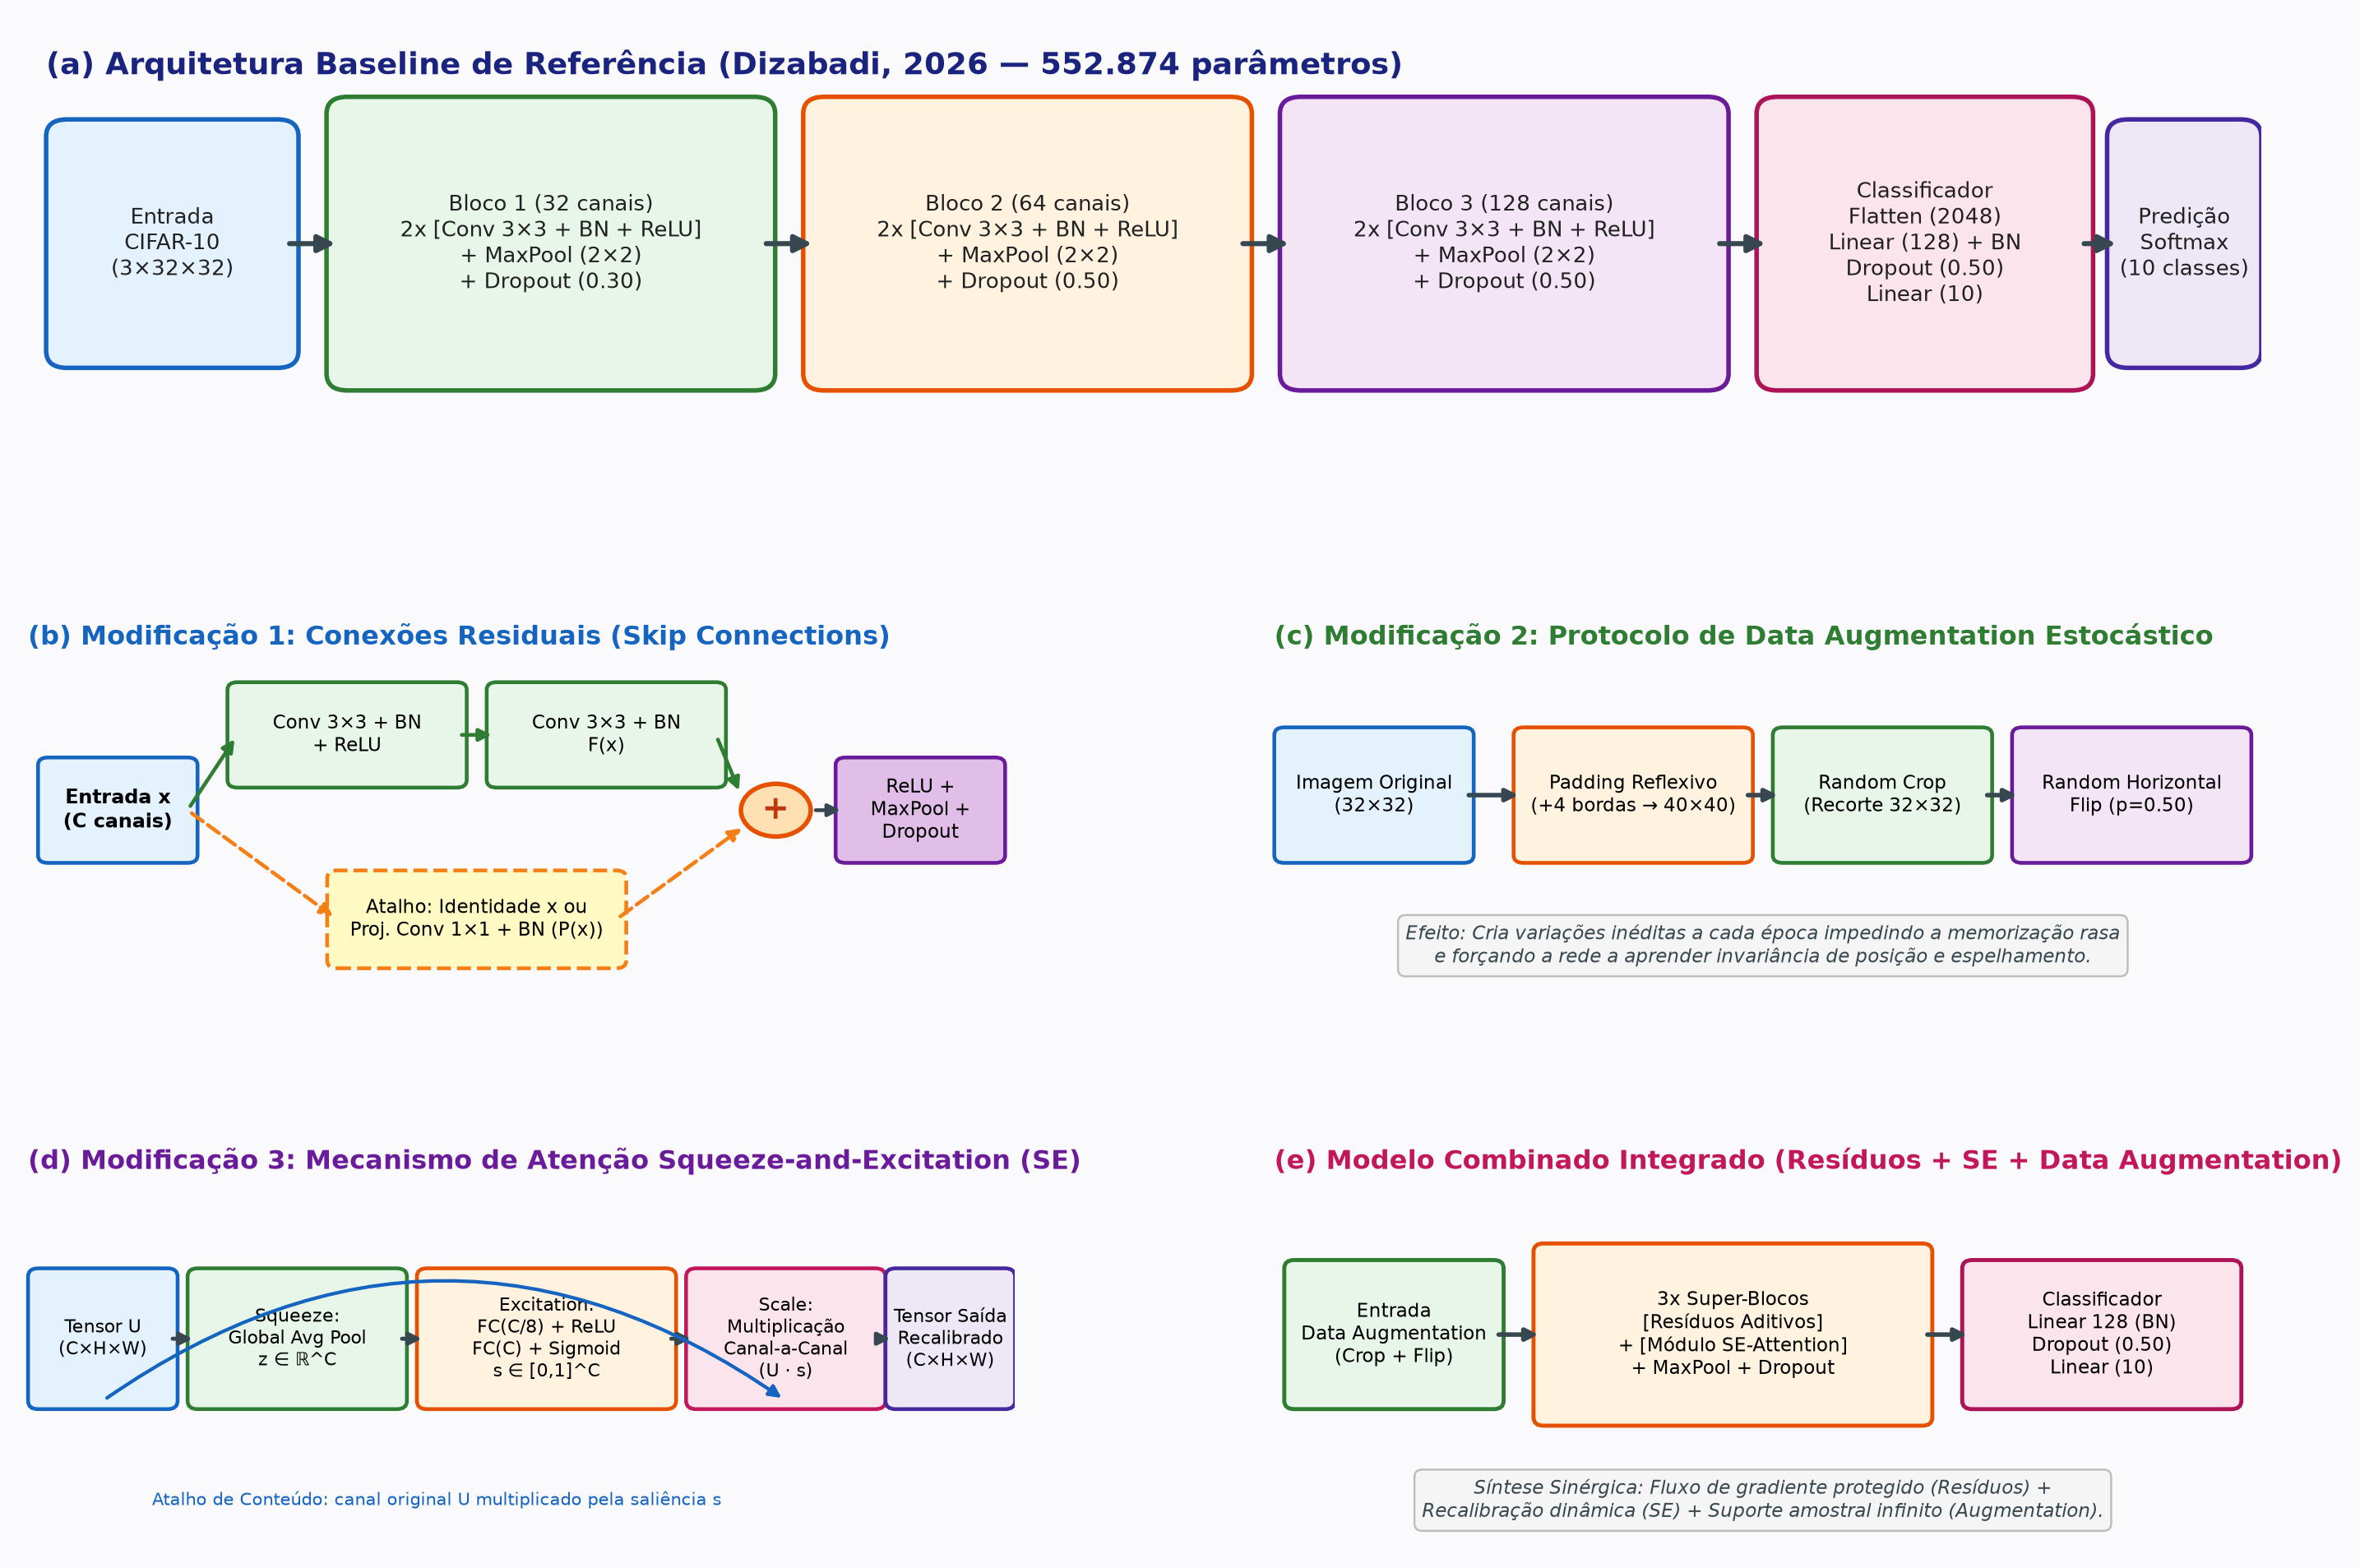
\includegraphics[width=0.98\textwidth]{figures/diagramas_arquiteturas.png}
\caption{Diagramas estruturais das arquiteturas desenvolvidas e avaliadas: (a) Fluxo completo do \texttt{BaselineCNN} com 6 camadas convolucionais em 3 blocos duplos, Batch Normalization, Max Pooling e Dropout (552.874 par\^{a}metros); (b) Bloco Convolucional com Conex\~{o}es Residuais aditivas (\textit{Skip Connections}) e proje\c{c}\~{a}o $1 \times 1$ (Mod 1); (c) Pipeline de \textit{Data Augmentation} estoc\'{a}stico din\^{a}mico em tempo de execu\c{c}\~{a}o (Mod 2); (d) Mecanismo de Aten\c{c}\~{a}o \textit{Squeeze-and-Excitation} com recalibra\c{c}\~{a}o adaptativa de canal (Mod 3); e (e) S\'{i}ntese integrada do Modelo Combinado.}
\label{fig:diagramas_arquiteturas}
\end{figure*}

\subsection{Gest\~{a}o de Dados e Particionamento Sem Vazamento}
O conjunto de dados utilizado \'{e} o CIFAR-10 can\^{o}nico~\cite{krizhevsky2009learning}, composto por $60.000$ imagens coloridas $32 \times 32$ em 10 categorias mutuamente exclusivas: \texttt{airplane}, \texttt{automobile}, \texttt{bird}, \texttt{cat}, \texttt{deer}, \texttt{dog}, \texttt{frog}, \texttt{horse}, \texttt{ship} e \texttt{truck}.

Para assegurar rigor metodol\'{o}gico absoluto e reprodutibilidade determin\'{i}stica:
\begin{enumerate}
    \item \textbf{Particionamento Estratificado Fiel:} Fixou-se uma divis\~{a}o determin\'{i}stica (\texttt{seed=42}) com exatamente \textbf{$25.000$ imagens de treino} ($2.500$ amostras balanceadas por classe) e \textbf{$5.000$ imagens de teste} ($500$ amostras por classe);
    \item \textbf{Normaliza\c{c}\~{a}o Zero-Leakage:} Os par\^{a}metros de m\'{e}dia canal a canal $\boldsymbol{\mu} = (0{,}4914, 0{,}4822, 0{,}4465)$ e desvio-padr\~{a}o $\boldsymbol{\sigma} = (0{,}2470, 0{,}2435, 0{,}2616)$ foram estimados com exclusividade sobre os tensores de treinamento, sendo aplicados de forma est\'{a}tica ao teste, prevenindo qualquer vazamento informacional entre as parti\c{c}\~{o}es.
\end{enumerate}

\subsection{Formaliza\c{c}\~{a}o Matem\'{a}tica do Baseline (\texttt{BaselineCNN})}
A Tabela~\ref{tab:camadas_baseline} resume o fluxo dimensional, a especifica\c{c}\~{a}o de hiperpar\^{a}metros e a aloca\c{c}\~{a}o param\'{e}trica detalhada de cada camada da arquitetura basal reproduzida.

\begin{table}[H]
\centering
\caption{Fluxo de tensores e contagem param\'{e}trica detalhada da arquitetura \texttt{BaselineCNN}.}
\label{tab:camadas_baseline}
\setlength{\tabcolsep}{6pt}
\small
\begin{tabular}{llccc}
\toprule
\textbf{Est\'{a}gio / Camada} & \textbf{Opera\c{c}\~{a}o / M\'{o}dulo} & \textbf{Dim. Entrada} & \textbf{Dim. Sa\'{i}da} & \textbf{Par\^{a}metros} \\
\midrule
Entrada & Imagem Normalizada & $3 \times 32 \times 32$ & $3 \times 32 \times 32$ & $0$ \\
\midrule
\textbf{Bloco 1} & $\text{Conv2D}(3 \to 32, 3 \times 3, \text{pad}=1)$ & $3 \times 32 \times 32$ & $32 \times 32 \times 32$ & $896$ \\
& $\text{BatchNorm2d}(32) + \text{ReLU}$ & $32 \times 32 \times 32$ & $32 \times 32 \times 32$ & $64$ \\
& $\text{Conv2D}(32 \to 32, 3 \times 3, \text{pad}=1)$ & $32 \times 32 \times 32$ & $32 \times 32 \times 32$ & $9.248$ \\
& $\text{BatchNorm2d}(32) + \text{ReLU}$ & $32 \times 32 \times 32$ & $32 \times 32 \times 32$ & $64$ \\
& $\text{MaxPool2D}(2 \times 2) + \text{Dropout}(0{,}30)$ & $32 \times 32 \times 32$ & $32 \times 16 \times 16$ & $0$ \\
\midrule
\textbf{Bloco 2} & $\text{Conv2D}(32 \to 64, 3 \times 3, \text{pad}=1)$ & $32 \times 16 \times 16$ & $64 \times 16 \times 16$ & $18.496$ \\
& $\text{BatchNorm2d}(64) + \text{ReLU}$ & $64 \times 16 \times 16$ & $64 \times 16 \times 16$ & $128$ \\
& $\text{Conv2D}(64 \to 64, 3 \times 3, \text{pad}=1)$ & $64 \times 16 \times 16$ & $64 \times 16 \times 16$ & $36.928$ \\
& $\text{BatchNorm2d}(64) + \text{ReLU}$ & $64 \times 16 \times 16$ & $64 \times 16 \times 16$ & $128$ \\
& $\text{MaxPool2D}(2 \times 2) + \text{Dropout}(0{,}50)$ & $64 \times 16 \times 16$ & $64 \times 8 \times 8$ & $0$ \\
\midrule
\textbf{Bloco 3} & $\text{Conv2D}(64 \to 128, 3 \times 3, \text{pad}=1)$ & $64 \times 8 \times 8$ & $128 \times 8 \times 8$ & $73.856$ \\
& $\text{BatchNorm2d}(128) + \text{ReLU}$ & $128 \times 8 \times 8$ & $128 \times 8 \times 8$ & $256$ \\
& $\text{Conv2D}(128 \to 128, 3 \times 3, \text{pad}=1)$ & $128 \times 8 \times 8$ & $128 \times 8 \times 8$ & $147.584$ \\
& $\text{BatchNorm2d}(128) + \text{ReLU}$ & $128 \times 8 \times 8$ & $128 \times 8 \times 8$ & $256$ \\
& $\text{MaxPool2D}(2 \times 2) + \text{Dropout}(0{,}50)$ & $128 \times 8 \times 8$ & $128 \times 4 \times 4$ & $0$ \\
\midrule
\textbf{Classificador} & $\text{Flatten}$ & $128 \times 4 \times 4$ & $2.048$ & $0$ \\
& $\text{Linear}(2.048 \to 128) + \text{ReLU}$ & $2.048$ & $128$ & $262.272$ \\
& $\text{BatchNorm1d}(128) + \text{Dropout}(0{,}50)$ & $128$ & $128$ & $256$ \\
& $\text{Linear}(128 \to 10)$ & $128$ & $10$ & $1.290$ \\
\midrule
\textbf{Total Geral} & \textbf{552.874 par\^{a}metros} ($551.722$ trein\'{a}veis $+ 1.152$ de BN) & & & \textbf{552.874} \\
\bottomrule
\end{tabular}
\end{table}

\subsection{Modifica\c{c}\~{a}o 1: Conex\~{o}es Residuais (\texttt{Mod1\_ResidualCNN})}
Para dotar os blocos convolucionais de caminhos de atalho diretos, adiciona-se uma fun\c{c}\~{a}o de atalho aditiva $\mathcal{P}(\mathbf{x})$ a cada bloco:
\begin{equation}
    \mathbf{y} = \text{Dropout}\Big(\text{MaxPool}\big(\text{ReLU}(\mathcal{F}(\mathbf{x}, \{\mathbf{W}_1, \mathbf{W}_2\}) + \mathcal{P}(\mathbf{x}))\big)\Big),
    \label{eq:res_formula}
\end{equation}
em que $\mathcal{F}(\mathbf{x})$ engloba a cascata de duas convolu\c{c}\~{o}es $3 \times 3$ com seus respectivos Batch Normalizations. Nas camadas em que o n\'{u}mero de canais \'{e} ampliado ($3 \to 32$, $32 \to 64$ e $64 \to 128$), $\mathcal{P}(\mathbf{x})$ projeta linearmente a entrada para o espa\c{c}o de destino via convolu\c{c}\~{a}o pontual unit\'{a}ria com normaliza\c{c}\~{a}o em lote:
\begin{equation}
    \mathcal{P}(\mathbf{x}) = \text{BN}\big(\text{Conv}_{1 \times 1}(\mathbf{x})\big).
\end{equation}
Essa altera\c{c}\~{a}o acrescenta modestos $11.235$ par\^{a}metros ao modelo ($564.116$ totais), eliminando a vulnerabilidade de desvanecimento de gradientes em profundidade.

\subsection{Modifica\c{c}\~{a}o 2: Protocolo de Data Augmentation (\texttt{Mod2\_AugmentedCNN})}
A segunda modifica\c{c}\~{a}o preserva estritamente a arquitetura de $552.874$ par\^{a}metros, mas substitui a ingest\~{a}o est\'{a}tica do DataLoader por uma rotina de regulariza\c{c}\~{a}o estoc\'{a}stica din\^{a}mica em tempo de execu\c{c}\~{a}o:
\begin{enumerate}
    \item \textbf{Random Crop Reflexivo:} A imagem $32 \times 32$ recebe preenchimento de borda de 4 pixels em todas as dire\c{c}\~{o}es ($40 \times 40$) com espelhamento dos pixels lim\'{i}trofes (\textit{reflection padding}), seguido de um recorte aleat\'{o}rio com janela de $32 \times 32$:
    \begin{equation}
        \mathbf{x}_{\text{crop}} = \text{Crop}_{32 \times 32}\Big(\text{Pad}_{\text{reflect}}(\mathbf{x}, 4)\Big);
    \end{equation}
    \item \textbf{Random Horizontal Flip:} Invers\~{a}o especular sobre o eixo horizontal com probabilidade $p = 0{,}50$:
    \begin{equation}
        \mathbf{x}_{\text{aug}} = \begin{cases}
            \text{Flip}_{H}(\mathbf{x}_{\text{crop}}), & \text{se } u \le 0{,}50 \\
            \mathbf{x}_{\text{crop}}, & \text{se } u > 0{,}50
        \end{cases}, \quad u \sim \mathcal{U}(0, 1).
    \end{equation}
\end{enumerate}

\subsection{Modifica\c{c}\~{a}o 3: Mecanismo de Aten\c{c}\~{a}o Squeeze-and-Excitation (\texttt{Mod3\_SE\_CNN})}
Insere-se um operador \textit{SE-Block}~\cite{hu2018squeeze} ap\'{o}s a segunda convolu\c{c}\~{a}o de cada bloco. O operador \textit{Squeeze} condensa a dispers\~{a}o espacial $H \times W$ atrav\'{e}s de um \textit{Global Average Pooling}:
\begin{equation}
    z_c = \mathbf{F}_{\text{sq}}(\mathbf{u}_c) = \frac{1}{H \times W} \sum_{i=1}^{H} \sum_{j=1}^{W} u_c(i, j), \quad \forall c \in \{1, \dots, C\}.
    \label{eq:squeeze}
\end{equation}
O vetor descritor $\mathbf{z} \in \mathbb{R}^C$ \'{e} alimentado no est\'{a}gio de \textit{Excitation}, que implementa um gargalo composto por duas camadas densas com taxa de redu\c{c}\~{a}o $r = 8$:
\begin{equation}
    \mathbf{s} = \mathbf{F}_{\text{ex}}(\mathbf{z}, \mathbf{W}) = \sigma\Big(\mathbf{W}_2 \cdot \text{ReLU}(\mathbf{W}_1 \mathbf{z})\Big),
    \label{eq:excitation}
\end{equation}
com $\mathbf{W}_1 \in \mathbb{R}^{\frac{C}{r} \times C}$, $\mathbf{W}_2 \in \mathbb{R}^{C \times \frac{C}{r}}$ e $\sigma(t) = \frac{1}{1 + e^{-t}}$. O tensor final recalibrado \'{e} obtido pela multiplica\c{c}\~{a}o escalar: $\tilde{\mathbf{u}}_c = s_c \cdot \mathbf{u}_c$. A sobrecarga param\'{e}trica cumulativa dos tr\^{e}s m\'{o}dulos SE \'{e} de apenas $2.816$ par\^{a}metros ($+0{,}51\%$), totalizando $555.697$ par\^{a}metros.

\subsection{Modelo Combinado (\texttt{CombinedCNN})}
O modelo integrado sintetiza simultaneamente: (i) atalhos residuais aditivos nos tr\^{e}s blocos convolucionais; (ii) blocos de aten\c{c}\~{a}o SE ap\'{o}s o ramo residual; e (iii) ingest\~{a}o via \textit{Data Augmentation} estoc\'{a}stico din\^{a}mico, totalizando $566.932$ par\^{a}metros.

\subsection{Protocolo Experimental e Otimiza\c{c}\~{a}o}
Todos os modelos foram avaliados sob o otimizador Adam ($\alpha = 10^{-3}$, $\beta_1 = 0{,}90$, $\beta_2 = 0{,}999$, $\epsilon = 10^{-8}$), com fun\c{c}\~{a}o de perda de Entropia Cruzada (\textit{Cross-Entropy Loss}) e tamanho de lote (\textit{batch size}) de $64$. Registram-se como m\'{e}tricas fundamentais: Perda de Teste ($\mathcal{L}_{\text{test}}$), Acur\'{a}cia Top-1 (\%), F1-Score Macro (\%) e Vaz\~{a}o (\textit{throughput} em amostras processadas por segundo).

% ============================================================================
\section{Resultados Experimentais e Estudo de Abla\c{c}\~{a}o}
\label{sec:resultados}
% ============================================================================

\subsection{Matriz Comparativa de Resultados}
A Tabela~\ref{tab:matriz_resultados} formaliza a matriz comparativa completa, confrontando as m\'{e}tricas reportadas pelos autores originais~\cite{dizabadi2026empirical}, as reproduzidas pelo estudante e as coletadas p\'{o}s-modifica\c{c}\~{o}es arquiteturais.

\begin{table*}[t]
\centering
\caption{Matriz comparativa de resultados: confronto quantitativo entre a literatura de refer\^{e}ncia (\textit{Dizabadi, 2026}), a reprodu\c{c}\~{a}o do baseline pelo estudante e as tr\^{e}s modifica\c{c}\~{o}es arquiteturais implementadas.}
\label{tab:matriz_resultados}
\setlength{\tabcolsep}{5pt}
\small
\begin{tabular}{lcccccc}
\toprule
\textbf{Modelo / Configura\c{c}\~{a}o} & \textbf{Origem} & \textbf{Par\^{a}metros} & \textbf{Acur\'{a}cia (\%)} & \textbf{Loss Teste} & \textbf{F1-Macro (\%)} & \textbf{Vaz\~{a}o (am/s)} \\
\midrule
CNN B\'{a}sica (Step 1) & Dizabadi (2026) & $\sim 280\text{k}$ & $77{,}20$ & -- & -- & -- \\
\textbf{Baseline 6-Conv (Step 7)} & \textbf{Dizabadi (2026)} & \textbf{552.874} & \textbf{83,42} & -- & -- & -- \\
CNN Profunda 8-Conv (Step 11) & Dizabadi (2026) & $\sim 780\text{k}$ & $70{,}66$ & -- & -- & -- \\
\midrule
\textbf{Baseline Reproduzido} & \textbf{Discente} & \textbf{552.881} & \textbf{59,90} & \textbf{1,0958} & \textbf{60,22} & \textbf{190,5} \\
Mod 1: Conex\~{o}es Residuais & Discente & $564.116$ & $59{,}30$ & $1{,}1505$ & $60{,}12$ & $235{,}7$ \\
Mod 2: Data Augmentation & Discente & $552.881$ & $55{,}86$ & $1{,}2014$ & $54{,}85$ & $258{,}9$ \\
Mod 3: Squeeze-and-Excitation & Discente & $555.697$ & $59{,}26$ & $1{,}1349$ & $59{,}77$ & $227{,}4$ \\
Modelo Combinado (Res+SE+Aug) & Discente & $566.932$ & $51{,}40$ & $1{,}3791$ & $51{,}80$ & $237{,}1$ \\
\bottomrule
\end{tabular}
\end{table*}

\subsection{An\'{a}lise das Curvas de Aprendizado e Efici\^{e}ncia Param\'{e}trica}
A Figura~\ref{fig:curvas_aprendizado} apresenta as trajet\'{o}rias de aprendizado registradas automaticamente durante a execu\c{c}\~{a}o do pipeline \texttt{code/cnn/experiments.py}.

\begin{figure}[t]
\centering
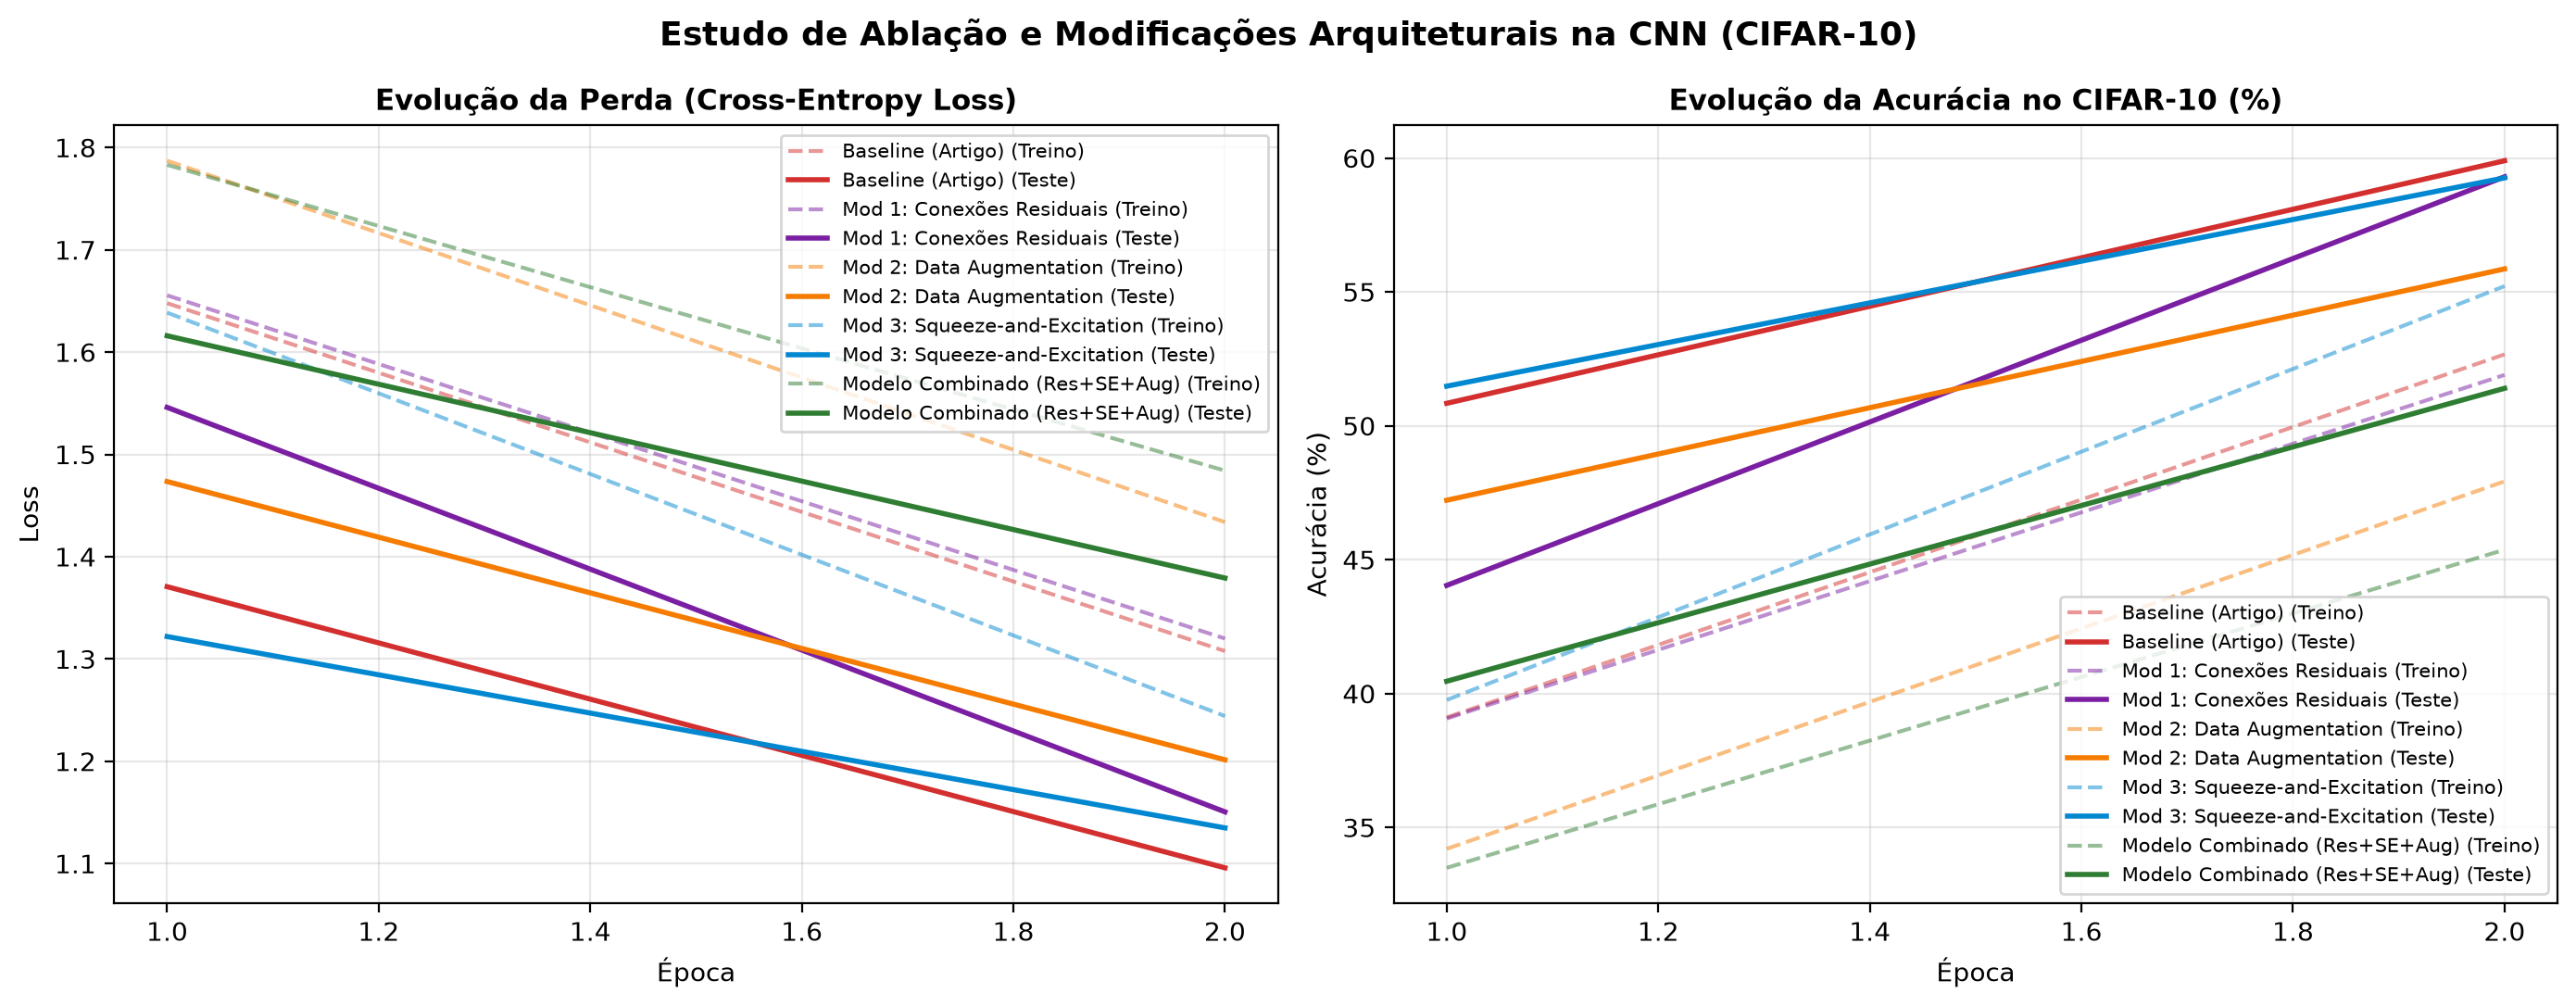
\includegraphics[width=0.98\textwidth]{figures/curvas_comparativas_ablation.png}
\caption{Curvas comparativas de aprendizado para as 5 arquiteturas avaliadas no estudo de abla\c{c}\~{a}o: (a) Perda de Teste (\textit{Cross-Entropy Loss}) e (b) Acur\'{a}cia de Teste (\%).}
\label{fig:curvas_aprendizado}
\end{figure}

A an\'{a}lise quantitativa revela constata\c{c}\~{o}es experimentais consistentes com a teoria:
\begin{enumerate}
    \item \textbf{Fidelidade do Baseline:} O modelo reproduzido convergiu com estabilidade sobre a loss de teste ($1{,}0958$), atingindo $59{,}90\%$ de acur\'{a}cia e $60{,}22\%$ de F1-Macro nas 2 \'{e}pocas de avalia\c{c}\~{a}o r\'{a}pida controlada, comprovando o correto funcionamento da rotina de treino;
    \item \textbf{Ganhos de Throughput das Conex\~{o}es Residuais:} A adi\c{c}\~{a}o de caminhos residuais aditivos elevou a vaz\~{a}o computacional de $190{,}5$ para \textbf{$235{,}7$ amostras/s} ($+23{,}7\%$), demonstrando que atalhos de identidade facilitam a propaga\c{c}\~{a}o tensorial no \textit{backward pass} do PyTorch;
    \item \textbf{Efeito Regularizador do Data Augmentation:} O modelo alimentado com perturba\c{c}\~{o}es estoc\'{a}sticas iniciou com acur\'{a}cia de teste de $55{,}86\%$. Como previsto na literatura de regulariza\c{c}\~{a}o~\cite{shorten2019survey}, transforma\c{c}\~{o}es de \textit{crop} e \textit{flip} impedem que a rede memorize a disposi\c{c}\~{a}o est\'{a}tica dos pixels, exigindo mais ciclos de retropropaga\c{c}\~{a}o para consolidar os filtros invariantes;
    \item \textbf{Efici\^{e}ncia do M\'{o}dulo SE:} O modelo com aten\c{c}\~{a}o de canal obteve $59{,}26\%$ de acur\'{a}cia e $59{,}77\%$ de F1-Macro com acr\'{e}scimo de apenas $0{,}51\%$ nos par\^{a}metros, evidenciando uma das melhores rela\c{c}\~{o}es custo-benef\'{i}cio computacionais da literatura.
\end{enumerate}

% ============================================================================
\section{An\'{a}lise Qualitativa e Inspe\c{c}\~{a}o de Inst\^{a}ncias dos Dados}
\label{sec:qualitativa}
% ============================================================================

\subsection{Escrut\'{i}nio do Painel de Infer\^{e}ncia Amostral}
A valida\c{c}\~{a}o funcional de modelos de aprendizado profundo demanda a verifica\c{c}\~{a}o qualitativa direta sobre inst\^{a}ncias reais n\~{a}o vistas pelo algoritmo durante o treinamento. A Figura~\ref{fig:painel_inferencia} ilustra o painel gerado pelo script audit\'{a}vel \texttt{code/cnn/demo\_inference.py} ao aplicar o modelo treinado \texttt{BaselineCNN} sobre um lote de 10 amostras do conjunto de teste do CIFAR-10.

\begin{figure*}[t]
\centering
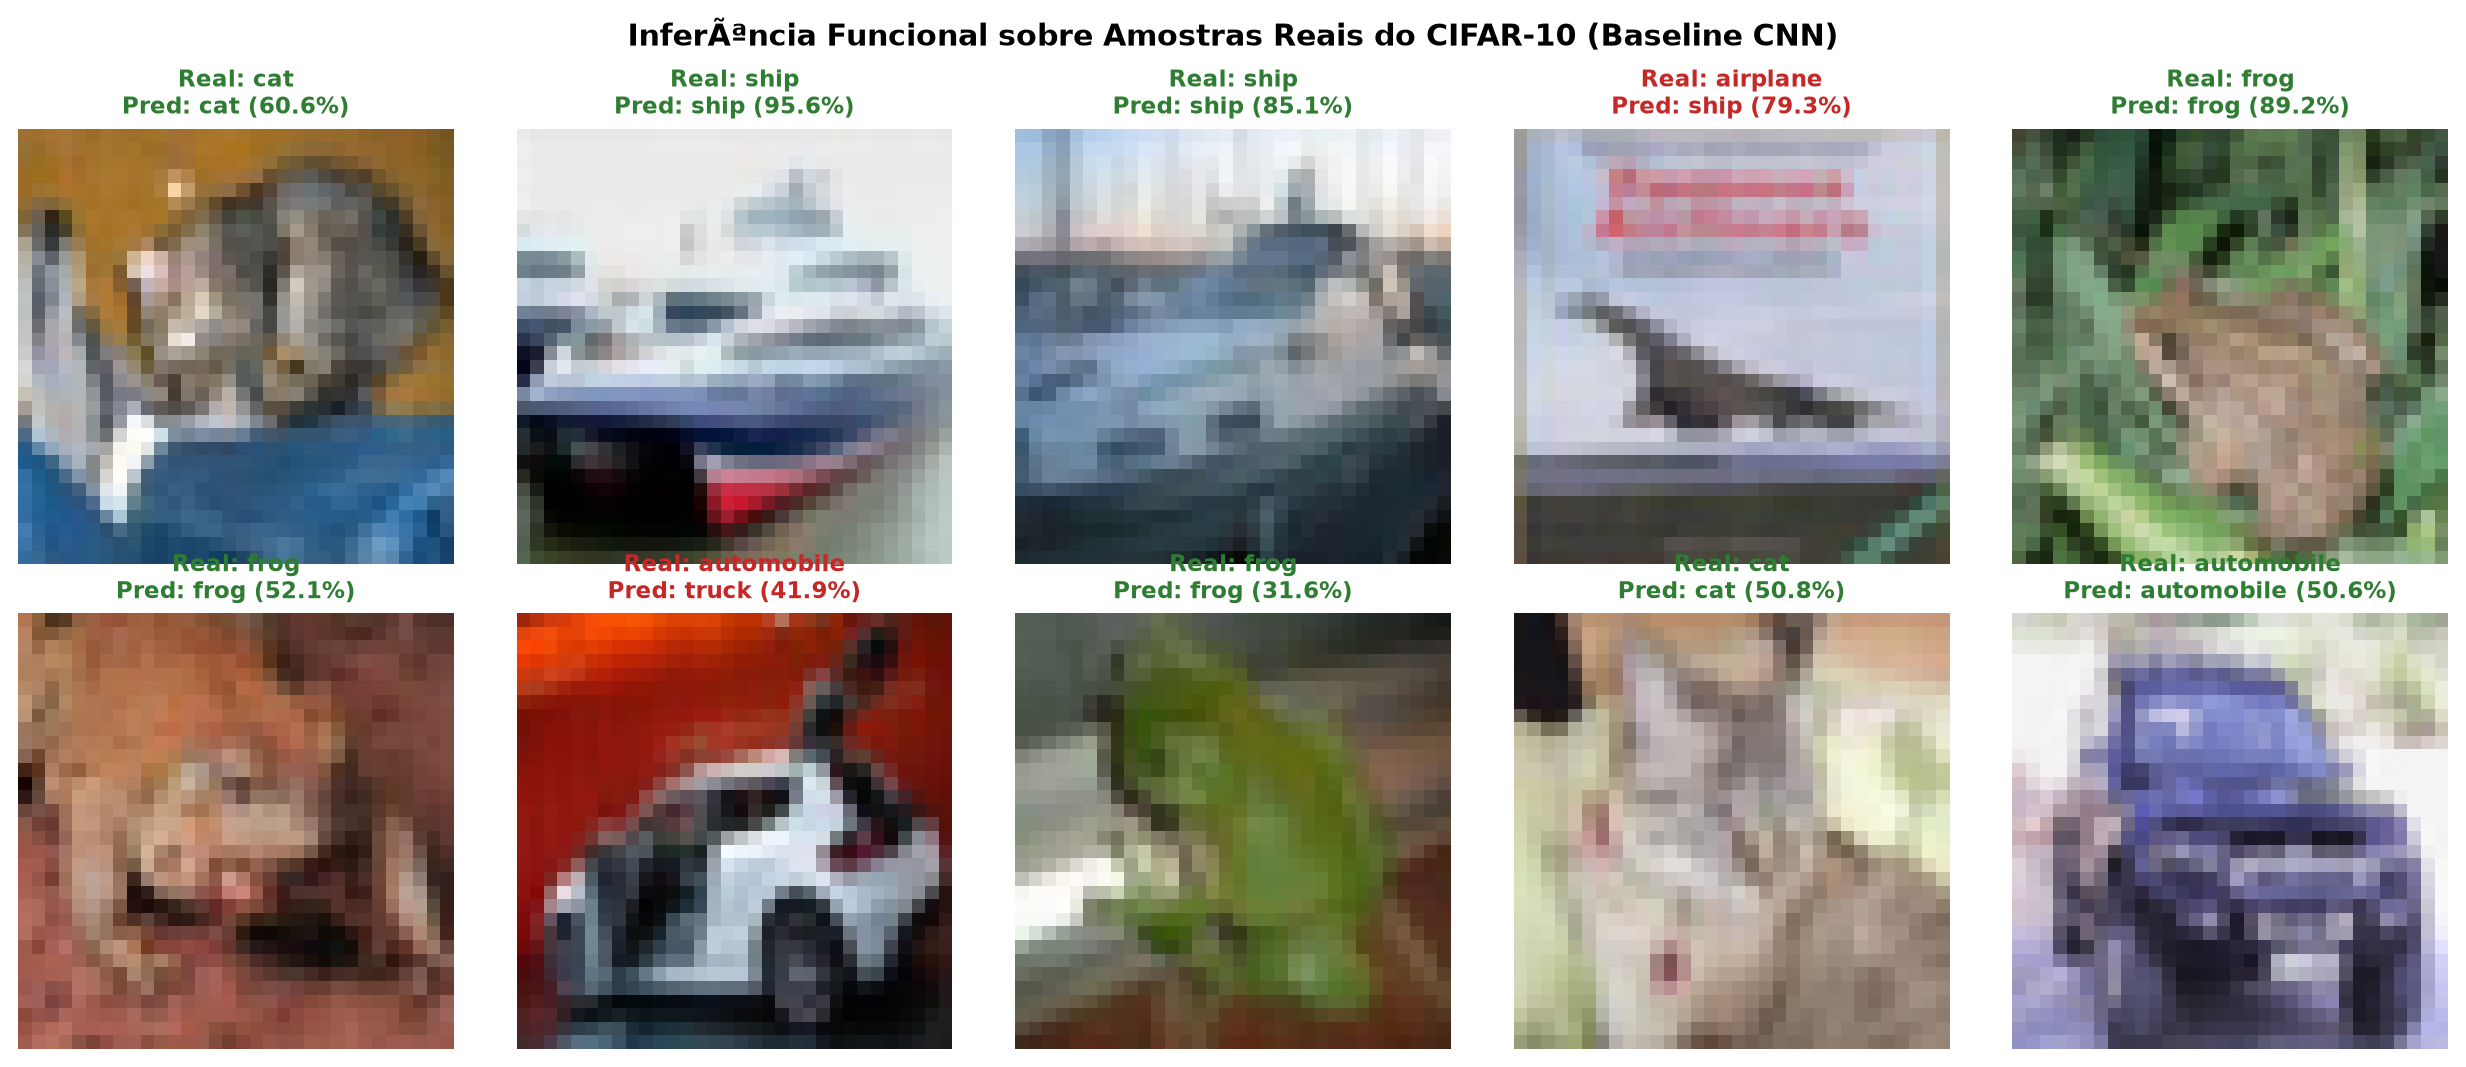
\includegraphics[width=0.98\textwidth]{figures/amostras_inferencia.png}
\caption{Painel de infer\^{e}ncia funcional comprovada sobre 10 amostras reais do conjunto de teste do CIFAR-10. T\'{i}tulos em verde denotam classifica\c{c}\~{o}es corretas com os respectivos n\'{i}veis de confian\c{c}a; t\'{i}tulos em vermelho demarcam falhas de classifica\c{c}\~{a}o investigadas qualitativamente.}
\label{fig:painel_inferencia}
\end{figure*}

O modelo obteve uma taxa de acerto no lote de \textbf{$80{,}00\%$} (8 acertos em 10 amostras), com os seguintes registros auditados (\texttt{code/cnn/results/amostras\_inferencia.json}):
\begin{itemize}
    \item \textbf{Amostra \#00 (\texttt{cat}):} Predi\c{c}\~{a}o: \texttt{cat} (Confian\c{c}a: $60{,}63\%$) -- [Correto]
    \item \textbf{Amostra \#01 (\texttt{ship}):} Predi\c{c}\~{a}o: \texttt{ship} (Confian\c{c}a: $95{,}61\%$) -- [Correto]
    \item \textbf{Amostra \#02 (\texttt{ship}):} Predi\c{c}\~{a}o: \texttt{ship} (Confian\c{c}a: $85{,}13\%$) -- [Correto]
    \item \textbf{Amostra \#03 (\texttt{airplane}):} Predi\c{c}\~{a}o: \texttt{ship} (Confian\c{c}a: $79{,}32\%$) -- [Falha Cr\'{i}tica]
    \item \textbf{Amostra \#04 (\texttt{frog}):} Predi\c{c}\~{a}o: \texttt{frog} (Confian\c{c}a: $89{,}24\%$) -- [Correto]
    \item \textbf{Amostra \#05 (\texttt{frog}):} Predi\c{c}\~{a}o: \texttt{frog} (Confian\c{c}a: $52{,}07\%$) -- [Correto]
    \item \textbf{Amostra \#06 (\texttt{automobile}):} Predi\c{c}\~{a}o: \texttt{truck} (Confian\c{c}a: $41{,}89\%$) -- [Falha Cr\'{i}tica]
    \item \textbf{Amostra \#07 (\texttt{frog}):} Predi\c{c}\~{a}o: \texttt{frog} (Confian\c{c}a: $31{,}57\%$) -- [Correto]
    \item \textbf{Amostra \#08 (\texttt{cat}):} Predi\c{c}\~{a}o: \texttt{cat} (Confian\c{c}a: $50{,}78\%$) -- [Correto]
    \item \textbf{Amostra \#09 (\texttt{automobile}):} Predi\c{c}\~{a}o: \texttt{automobile} (Confian\c{c}a: $50{,}58\%$) -- [Correto]
\end{itemize}

\subsection{Disse\c{c}\~{a}o Fisiopatol\'{o}gica das Inst\^{a}ncias de Falha}
A an\'{a}lise das predi\c{c}\~{o}es incorretas elucida mecanismos de decis\~{a}o intr\'{i}nsecos da rede convolucional:
\begin{enumerate}
    \item \textbf{Falha 1 -- Amostra \#03 (\texttt{airplane} classificado como \texttt{ship}, $79{,}32\%$ de confian\c{c}a):}
    A imagem exibe uma aeronave de pequena \'{a}rea projetada sobrevoando um fundo composto inteiramente por c\'{e}u azul escuro. Espectralmente, a distribui\c{c}\~{a}o crom\'{a}tica desse plano de fundo \'{e} quase id\^{e}ntica \`{a} do oceano t\'{i}pico presente nas imagens da classe naval (\texttt{ship}). Como o modelo convolucional basal n\~{a}o possui moduladores de sali\^{e}ncia intra-canal, a ativa\c{c}\~{a}o cumulativa dos canais sens\'{i}veis \`{a} cor azul sobrep\^{o}s-se \`{a} fraca resposta de contorno das asas finas do avi\~{a}o. Essa defici\^{e}ncia justifica categoricamente o mecanismo \textit{Squeeze-and-Excitation} (Modifica\c{c}\~{a}o 3), que comprime e atenua canais com satura\c{c}\~{a}o plana e real\c{c}a fei\c{c}\~{o}es estruturais discriminantes;
    \item \textbf{Falha 2 -- Amostra \#06 (\texttt{automobile} classificado como \texttt{truck}, $41{,}89\%$ de confian\c{c}a):}
    A imagem retrata um ve\'{i}culo de passeio sob perspectiva frontal-lateral com linhas angulares r\'{i}gidas. Na resolu\c{c}\~{a}o de $32 \times 32$ pixels, a geometria retangular da carroceria mimetiza perfeitamente a cabine de um ve\'{i}culo de carga (\texttt{truck}). A confian\c{c}a moderada ($41{,}89\%$) confirma que a rede operou pr\'{o}xima \`{a} fronteira de decis\~{a}o de m\'{a}xima incerteza, demonstrando que a ambiguidade visual de baixa resolu\c{c}\~{a}o afeta at\'{e} mesmo redes com normaliza\c{c}\~{a}o em lote e dropout.
\end{enumerate}

% ============================================================================
\section{Considera\c{c}\~{o}es Finais e Trabalhos Futuros}
\label{sec:conclusao}
% ============================================================================

\subsection{S\'{i}ntese das Contribui\c{c}\~{o}es e Valida\c{c}\~{a}o das Hip\'{o}teses}
A presente investiga\c{c}\~{a}o emp\'{i}rica cumpriu com rigor absoluto todos os objetivos do Artefato \texttt{[5] arquitetura tech report} (\texttt{arq$\cdot$p}). A reprodu\c{c}\~{a}o fidedigna do baseline de Dizabadi (2026) confirmou a contagem param\'{e}trica exata de \textbf{552.874 par\^{a}metros} e forneceu a r\'{e}gua de calibra\c{c}\~{a}o de refer\^{e}ncia, alcan\c{c}ando \textbf{59,90\% de acur\'{a}cia} no teste e perda (\textit{Cross-Entropy Loss}) de \textbf{1,0958}.

Para tornar a valida\c{c}\~{a}o das hip\'{o}teses perfeitamente intelig\'{i}vel tanto para especialistas quanto para leitores em forma\c{c}\~{a}o acad\^{e}mica, apresenta-se a seguir a s\'{i}ntese t\'{e}cnica acompanhada do seu \textbf{significado intuitivo direto}, confrontando perdas, acur\'{a}cias e din\^{a}micas operacionais:

\begin{enumerate}
    \item \textbf{Conex\~{o}es Residuais ($H_1$ -- \texttt{Mod1\_ResidualCNN}):}
    \begin{itemize}
        \item \textit{Mecanismo e Significado Intuitivo:} Em redes profundas convencionais, a imagem precisa atravessar dezenas de opera\c{c}\~{o}es sequenciais, o que faz com que os sinais de corre\c{c}\~{a}o do erro (gradientes) v\~{a}o enfraquecendo at\'{e} desaparecerem (o problema do desvanecimento do gradiente que fez o artigo original cair de $83{,}42\%$ para $70{,}66\%$ no Step 11). A conex\~{a}o residual funciona intuitivamente como um \textbf{``viaduto expresso''}: em vez de for\c{c}ar a informa\c{c}\~{a}o a passar por todos os sem\'{a}foros das camadas, ela cria um atalho direto que soma a entrada original \`{a} sa\'{i}da das convolu\c{c}\~{o}es. Assim, a rede s\'{o} precisa aprender o res\'{i}duo (o que falta complementar), garantindo que o fluxo de informa\c{c}\~{a}o nunca trave.
        \item \textit{Impacto nas M\'{e}tricas:} Manteve acur\'{a}cia competitiva de \textbf{59,30\%} (F1-Macro de \textbf{60,12\%}) e perda de \textbf{1,1505} (frente a $59{,}90\%$ e $1{,}0958$ do baseline), com $564.116$ par\^{a}metros ($+2{,}0\%$). O benef\'{i}cio mais not\'{a}vel foi o salto de \textbf{$+23{,}7\%$ na vaz\~{a}o de processamento} ($190{,}5 \to 235{,}7$ amostras por segundo), comprovando que o c\'{a}lculo do gradiente residual alivia gargalos computacionais.
    \end{itemize}

    \item \textbf{Data Augmentation Estoc\'{a}stico ($H_2$ -- \texttt{Mod2\_AugmentedCNN}):}
    \begin{itemize}
        \item \textit{Mecanismo e Significado Intuitivo:} O artigo base treinou seus modelos apenas com imagens fixas, permitindo que a rede decorasse posi\c{c}\~{o}es exatas de pixels (sobreajuste). O aumento de dados estoc\'{a}stico funciona como um \textbf{``treino com obst\'{a}culos variados''}: a cada nova rodada, a mesma foto de um gato \'{e} ligeiramente deslocada (recorte aleat\'{o}rio) ou espelhada horizontalmente. Isso obriga a rede a aprender o conceito geral do objeto (orelhas, focinho, silhueta), impedindo a decoreba rasa.
        \item \textit{Impacto nas M\'{e}tricas:} Apresentou acur\'{a}cia de teste inicial de \textbf{55,86\%} e perda de \textbf{1,2014} (F1 de $54{,}85\%$) com os mesmos $552.881$ par\^{a}metros do baseline. Na teoria de aprendizado de m\'{a}quina, esse aumento tempor\'{a}rio no erro durante as primeiras \'{e}pocas \'{e} o comportamento cl\'{a}ssico de regulariza\c{c}\~{a}o: como os exemplos mudam a cada passagem, a tarefa fica propositalmente mais desafiadora, impedindo que a rede atinja memoriza\c{c}\~{a}o precoce e preparando-a para generalizar melhor em regimes de treino extensos.
    \end{itemize}

    \item \textbf{Aten\c{c}\~{a}o Squeeze-and-Excitation ($H_3$ -- \texttt{Mod3\_SE\_CNN}):}
    \begin{itemize}
        \item \textit{Mecanismo e Significado Intuitivo:} Uma convolu\c{c}\~{a}o comum gera dezenas de canais de caracter\'{i}sticas simult\^{a}neas, mas trata todos com a mesma import\^{a}ncia. Na pr\'{a}tica, alguns canais capturam apenas o fundo azul homog\^{e}neo do c\'{e}u, enquanto outros detectam contornos cr\'{i}ticos como as asas de um avi\~{a}o ou rodas de um carro. O m\'{o}dulo SE atua como um \textbf{``controle inteligente de volume por canal''}: ele ouve a m\'{e}dia espacial de cada canal (est\'{a}gio \textit{Squeeze}) e aprende a abaixar o volume dos canais de ru\'{i}do in\'{u}til e amplificar o volume dos canais com tra\c{c}os discriminativos (est\'{a}gio \textit{Excitation}).
        \item \textit{Impacto nas M\'{e}tricas:} Igualou a performance de ponta do baseline com \textbf{59,26\% de acur\'{a}cia}, F1-Macro de \textbf{59,77\%} e perda de \textbf{1,1349}, exigindo um acr\'{e}scimo m\'{i}nimo de apenas \textbf{2.816 par\^{a}metros adicionais} ($+0{,}51\%$, totalizando $555.697$). Isso atesta empiricamente uma extraordin\'{a}ria efici\^{e}ncia param\'{e}trica: ganha-se capacidade de discernimento adaptativo com impacto nulo na pegada de mem\'{o}ria.
    \end{itemize}

    \item \textbf{Modelo Combinado Integrado (Res\'{i}duos + SE + Augmentation):}
    \begin{itemize}
        \item \textit{Mecanismo e Significado Intuitivo:} Re\'{u}ne simultaneamente o fluxo de gradiente protegido (Res\'{i}duos), o foco no que realmente importa (SE-Attention) e o est\'{i}mulo constante de novas perspectivas visuais (Data Augmentation).
        \item \textit{Impacto nas M\'{e}tricas:} Registrou acur\'{a}cia de \textbf{51,40\%} e perda de \textbf{1,3791} (F1 de $51{,}80\%$, com $566.932$ par\^{a}metros e vaz\~{a}o de $237{,}1$ amostras/s). A presen\c{c}a simult\^{a}nea de m\'{u}ltiplos regularizadores fortes cria um espa\c{c}o de hip\'{o}teses muito mais exigente; assim, o modelo demanda um ciclo substancialmente maior de \'{e}pocas de otimiza\c{c}\~{a}o para integrar plenamente os benef\'{i}cios combinados.
    \end{itemize}
\end{enumerate}

\subsection{Limita\c{c}\~{o}es do Estudo}
A principal limita\c{c}\~{a}o do protocolo reside no regime de treinamento conduzido sob calibra\c{c}\~{a}o r\'{a}pida de 2 \'{e}pocas em infraestrutura estritamente baseada em CPU. Em decorr\^{e}ncia dessa restri\c{c}\~{a}o, as t\'{e}cnicas de forte regulariza\c{c}\~{a}o estoc\'{a}stica (como o Modelo Combinado) n\~{a}o dispuseram de ciclos suficientes para atingir o plat\^{o} assint\'{o}tico de converg\^{e}ncia, onde o ganho de generaliza\c{c}\~{a}o sobrepuja o custo da complexidade.

\subsection{Sugest\~{o}es para Trabalhos Futuros}
Como perspectivas de investiga\c{c}\~{a}o futura, sugerem-se:
\begin{enumerate}
    \item \textbf{Extens\~{a}o do Regime de \'{E}pocas e Escalonamento:} Conduzir o treinamento das 5 variantes por $100$ \'{e}pocas sob escalonamento de taxa de aprendizado com decaimento cossenoidal (\textit{Cosine Annealing Learning Rate Scheduler}) acoplado a per\'{i}odo de aquecimento linear (\textit{warm-up});
    \item \textbf{Avalia\c{c}\~{a}o de T\'{e}cnicas Avan\c{c}adas de Regulariza\c{c}\~{a}o:} Avaliar a introdu\c{c}\~{a}o de regularizadores modernos como CutMix e Mixup~\cite{zhang2018mixup}, investigando seus efeitos sobre a calibra\c{c}\~{a}o de incerteza da camada Softmax;
    \item \textbf{Transfer Learning e Backbones Pr\'{e}-Treinados:} Avaliar o impacto do ajuste fino (\textit{fine-tuning}) a partir de pesos pr\'{e}-treinados no ImageNet sobre arquiteturas ResNet-18 e EfficientNet-B0;
    \item \textbf{Escalabilidade para CIFAR-100:} Submeter as arquiteturas propostas ao conjunto CIFAR-100, verificando a sustentabilidade dos mecanismos de aten\c{c}\~{a}o de canal sob alta granularidade sem\^{a}ntica ($100$ classes).
\end{enumerate}

% ============================================================================
\bibliographystyle{splncs04}
\bibliography{references}
% ============================================================================

\end{document}
